\documentclass[twoside]{book}

% Packages required by doxygen
\usepackage{fixltx2e}
\usepackage{calc}
\usepackage{doxygen}
\usepackage[export]{adjustbox} % also loads graphicx
\usepackage{graphicx}
\usepackage[utf8]{inputenc}
\usepackage{makeidx}
\usepackage{multicol}
\usepackage{multirow}
\PassOptionsToPackage{warn}{textcomp}
\usepackage{textcomp}
\usepackage[nointegrals]{wasysym}
\usepackage[table]{xcolor}

% Font selection
\usepackage[T1]{fontenc}
\usepackage[scaled=.90]{helvet}
\usepackage{courier}
\usepackage{amssymb}
\usepackage{sectsty}
\renewcommand{\familydefault}{\sfdefault}
\allsectionsfont{%
  \fontseries{bc}\selectfont%
  \color{darkgray}%
}
\renewcommand{\DoxyLabelFont}{%
  \fontseries{bc}\selectfont%
  \color{darkgray}%
}
\newcommand{\+}{\discretionary{\mbox{\scriptsize$\hookleftarrow$}}{}{}}

% Page & text layout
\usepackage{geometry}
\geometry{%
  a4paper,%
  top=2.5cm,%
  bottom=2.5cm,%
  left=2.5cm,%
  right=2.5cm%
}
\tolerance=750
\hfuzz=15pt
\hbadness=750
\setlength{\emergencystretch}{15pt}
\setlength{\parindent}{0cm}
\setlength{\parskip}{3ex plus 2ex minus 2ex}
\makeatletter
\renewcommand{\paragraph}{%
  \@startsection{paragraph}{4}{0ex}{-1.0ex}{1.0ex}{%
    \normalfont\normalsize\bfseries\SS@parafont%
  }%
}
\renewcommand{\subparagraph}{%
  \@startsection{subparagraph}{5}{0ex}{-1.0ex}{1.0ex}{%
    \normalfont\normalsize\bfseries\SS@subparafont%
  }%
}
\makeatother

% Headers & footers
\usepackage{fancyhdr}
\pagestyle{fancyplain}
\fancyhead[LE]{\fancyplain{}{\bfseries\thepage}}
\fancyhead[CE]{\fancyplain{}{}}
\fancyhead[RE]{\fancyplain{}{\bfseries\leftmark}}
\fancyhead[LO]{\fancyplain{}{\bfseries\rightmark}}
\fancyhead[CO]{\fancyplain{}{}}
\fancyhead[RO]{\fancyplain{}{\bfseries\thepage}}
\fancyfoot[LE]{\fancyplain{}{}}
\fancyfoot[CE]{\fancyplain{}{}}
\fancyfoot[RE]{\fancyplain{}{\bfseries\scriptsize Generated by Doxygen }}
\fancyfoot[LO]{\fancyplain{}{\bfseries\scriptsize Generated by Doxygen }}
\fancyfoot[CO]{\fancyplain{}{}}
\fancyfoot[RO]{\fancyplain{}{}}
\renewcommand{\footrulewidth}{0.4pt}
\renewcommand{\chaptermark}[1]{%
  \markboth{#1}{}%
}
\renewcommand{\sectionmark}[1]{%
  \markright{\thesection\ #1}%
}

% Indices & bibliography
\usepackage{natbib}
\usepackage[titles]{tocloft}
\setcounter{tocdepth}{3}
\setcounter{secnumdepth}{5}
\makeindex

% Hyperlinks (required, but should be loaded last)
\usepackage{ifpdf}
\ifpdf
  \usepackage[pdftex,pagebackref=true]{hyperref}
\else
  \usepackage[ps2pdf,pagebackref=true]{hyperref}
\fi
\hypersetup{%
  colorlinks=true,%
  linkcolor=blue,%
  citecolor=blue,%
  unicode%
}

% Custom commands
\newcommand{\clearemptydoublepage}{%
  \newpage{\pagestyle{empty}\cleardoublepage}%
}

\usepackage{caption}
\captionsetup{labelsep=space,justification=centering,font={bf},singlelinecheck=off,skip=4pt,position=top}

%===== C O N T E N T S =====

\begin{document}

% Titlepage & ToC
\hypersetup{pageanchor=false,
             bookmarksnumbered=true,
             pdfencoding=unicode
            }
\pagenumbering{roman}
\begin{titlepage}
\vspace*{7cm}
\begin{center}%
{\Large Template }\\
\vspace*{1cm}
{\large Generated by Doxygen 1.8.11}\\
\end{center}
\end{titlepage}
\clearemptydoublepage
\tableofcontents
\clearemptydoublepage
\pagenumbering{arabic}
\hypersetup{pageanchor=true}

%--- Begin generated contents ---
\chapter{My Personal Index Page}
\label{index}\hypertarget{index}{}\begin{DoxyAuthor}{Author}
Martijn Krijnen 
\end{DoxyAuthor}
\begin{DoxyVersion}{Version}
1.\+0 
\end{DoxyVersion}
\hypertarget{index_intro}{}\section{Introduction}\label{index_intro}
This is a basic template for a R\+OS node. Please copy it and adapt to fit your application. \hypertarget{index_install}{}\section{Installation}\label{index_install}
\hypertarget{index_step1}{}\subsection{Step 1\+: catkin build}\label{index_step1}

\chapter{Namespace Index}
\section{Namespace List}
Here is a list of all namespaces with brief descriptions\+:\begin{DoxyCompactList}
\item\contentsline{section}{\hyperlink{namespacetemplate__node}{template\+\_\+node} }{\pageref{namespacetemplate__node}}{}
\end{DoxyCompactList}

\chapter{Class Index}
\section{Class List}
Here are the classes, structs, unions and interfaces with brief descriptions\+:\begin{DoxyCompactList}
\item\contentsline{section}{\hyperlink{classtemplate__node_1_1TemplateAlgorithms}{template\+\_\+node\+::\+Template\+Algorithms} }{\pageref{classtemplate__node_1_1TemplateAlgorithms}}{}
\item\contentsline{section}{\hyperlink{classtemplate__node_1_1TemplateNode}{template\+\_\+node\+::\+Template\+Node} }{\pageref{classtemplate__node_1_1TemplateNode}}{}
\end{DoxyCompactList}

\chapter{File Index}
\section{File List}
Here is a list of all files with brief descriptions\+:\begin{DoxyCompactList}
\item\contentsline{section}{/home/martijn/scatkin/src/template/include/template/\hyperlink{template__algorithms_8h}{template\+\_\+algorithms.\+h} }{\pageref{template__algorithms_8h}}{}
\item\contentsline{section}{/home/martijn/scatkin/src/template/include/template/\hyperlink{template__node_8h}{template\+\_\+node.\+h} }{\pageref{template__node_8h}}{}
\item\contentsline{section}{/home/martijn/scatkin/src/template/src/\hyperlink{template__algorithms_8cpp}{template\+\_\+algorithms.\+cpp} }{\pageref{template__algorithms_8cpp}}{}
\item\contentsline{section}{/home/martijn/scatkin/src/template/src/\hyperlink{template__main_8cpp}{template\+\_\+main.\+cpp} }{\pageref{template__main_8cpp}}{}
\item\contentsline{section}{/home/martijn/scatkin/src/template/src/\hyperlink{template__node_8cpp}{template\+\_\+node.\+cpp} }{\pageref{template__node_8cpp}}{}
\end{DoxyCompactList}

\chapter{Namespace Documentation}
\hypertarget{namespacetemplate__node}{}\section{template\+\_\+node Namespace Reference}
\label{namespacetemplate__node}\index{template\+\_\+node@{template\+\_\+node}}
\subsection*{Classes}
\begin{DoxyCompactItemize}
\item 
class \hyperlink{classtemplate__node_1_1TemplateAlgorithms}{Template\+Algorithms}
\item 
class \hyperlink{classtemplate__node_1_1TemplateNode}{Template\+Node}
\end{DoxyCompactItemize}

\chapter{Class Documentation}
\hypertarget{classtemplate__node_1_1TemplateAlgorithms}{}\section{template\+\_\+node\+:\+:Template\+Algorithms Class Reference}
\label{classtemplate__node_1_1TemplateAlgorithms}\index{template\+\_\+node\+::\+Template\+Algorithms@{template\+\_\+node\+::\+Template\+Algorithms}}


{\ttfamily \#include $<$template\+\_\+algorithms.\+h$>$}

\subsection*{Public Member Functions}
\begin{DoxyCompactItemize}
\item 
\hyperlink{classtemplate__node_1_1TemplateAlgorithms_a2ad25bcfe53d334ccb0e8a63d2130ba8}{Template\+Algorithms} ()
\begin{DoxyCompactList}\small\item\em Constructor. \end{DoxyCompactList}\item 
virtual \hyperlink{classtemplate__node_1_1TemplateAlgorithms_acbed3c42187d8d716514c4ae0267cdfe}{$\sim$\+Template\+Algorithms} ()
\begin{DoxyCompactList}\small\item\em Destructor. \end{DoxyCompactList}\item 
double \hyperlink{classtemplate__node_1_1TemplateAlgorithms_a9c05db2f35b90b44c7a055ea58d55d42}{Add} (double x, double y)
\begin{DoxyCompactList}\small\item\em Add\+: example function which adds two doubles. \end{DoxyCompactList}\end{DoxyCompactItemize}


\subsection{Detailed Description}
Main class for the node to handle the R\+OS interfacing. 

\subsection{Constructor \& Destructor Documentation}
\index{template\+\_\+node\+::\+Template\+Algorithms@{template\+\_\+node\+::\+Template\+Algorithms}!Template\+Algorithms@{Template\+Algorithms}}
\index{Template\+Algorithms@{Template\+Algorithms}!template\+\_\+node\+::\+Template\+Algorithms@{template\+\_\+node\+::\+Template\+Algorithms}}
\subsubsection[{\texorpdfstring{Template\+Algorithms()}{TemplateAlgorithms()}}]{\setlength{\rightskip}{0pt plus 5cm}template\+\_\+node\+::\+Template\+Algorithms\+::\+Template\+Algorithms (
\begin{DoxyParamCaption}
{}
\end{DoxyParamCaption}
)}\hypertarget{classtemplate__node_1_1TemplateAlgorithms_a2ad25bcfe53d334ccb0e8a63d2130ba8}{}\label{classtemplate__node_1_1TemplateAlgorithms_a2ad25bcfe53d334ccb0e8a63d2130ba8}


Constructor. 

default constructor\+: no arguments or effect \index{template\+\_\+node\+::\+Template\+Algorithms@{template\+\_\+node\+::\+Template\+Algorithms}!````~Template\+Algorithms@{$\sim$\+Template\+Algorithms}}
\index{````~Template\+Algorithms@{$\sim$\+Template\+Algorithms}!template\+\_\+node\+::\+Template\+Algorithms@{template\+\_\+node\+::\+Template\+Algorithms}}
\subsubsection[{\texorpdfstring{$\sim$\+Template\+Algorithms()}{~TemplateAlgorithms()}}]{\setlength{\rightskip}{0pt plus 5cm}template\+\_\+node\+::\+Template\+Algorithms\+::$\sim$\+Template\+Algorithms (
\begin{DoxyParamCaption}
{}
\end{DoxyParamCaption}
)\hspace{0.3cm}{\ttfamily [virtual]}}\hypertarget{classtemplate__node_1_1TemplateAlgorithms_acbed3c42187d8d716514c4ae0267cdfe}{}\label{classtemplate__node_1_1TemplateAlgorithms_acbed3c42187d8d716514c4ae0267cdfe}


Destructor. 

default destructor\+: no arguments or content 

\subsection{Member Function Documentation}
\index{template\+\_\+node\+::\+Template\+Algorithms@{template\+\_\+node\+::\+Template\+Algorithms}!Add@{Add}}
\index{Add@{Add}!template\+\_\+node\+::\+Template\+Algorithms@{template\+\_\+node\+::\+Template\+Algorithms}}
\subsubsection[{\texorpdfstring{Add(double x, double y)}{Add(double x, double y)}}]{\setlength{\rightskip}{0pt plus 5cm}double template\+\_\+node\+::\+Template\+Algorithms\+::\+Add (
\begin{DoxyParamCaption}
\item[{double}]{x, }
\item[{double}]{y}
\end{DoxyParamCaption}
)}\hypertarget{classtemplate__node_1_1TemplateAlgorithms_a9c05db2f35b90b44c7a055ea58d55d42}{}\label{classtemplate__node_1_1TemplateAlgorithms_a9c05db2f35b90b44c7a055ea58d55d42}


Add\+: example function which adds two doubles. 


\begin{DoxyParams}{Parameters}
{\em x} & First double to add. \\
\hline
{\em y} & Second double to add. \\
\hline
\end{DoxyParams}
\begin{DoxyReturn}{Returns}
The sum of both parameters.
\end{DoxyReturn}
This method uses a little-\/known variant of integer addition known as Sophocles\textquotesingle{} Scissors. It optimises the function\textquotesingle{}s performance on many platforms that we may or may not choose to target in the future.  make sure I implemented the algorithm correctly with some unit tests. 

The documentation for this class was generated from the following files\+:\begin{DoxyCompactItemize}
\item 
/home/martijn/scatkin/src/template/include/template/\hyperlink{template__algorithms_8h}{template\+\_\+algorithms.\+h}\item 
/home/martijn/scatkin/src/template/src/\hyperlink{template__algorithms_8cpp}{template\+\_\+algorithms.\+cpp}\end{DoxyCompactItemize}

\hypertarget{classtemplate__node_1_1TemplateNode}{}\section{template\+\_\+node\+:\+:Template\+Node Class Reference}
\label{classtemplate__node_1_1TemplateNode}\index{template\+\_\+node\+::\+Template\+Node@{template\+\_\+node\+::\+Template\+Node}}


{\ttfamily \#include $<$template\+\_\+node.\+h$>$}

\subsection*{Public Member Functions}
\begin{DoxyCompactItemize}
\item 
\hyperlink{classtemplate__node_1_1TemplateNode_a4747c3118482eb109592c8877a5c1139}{Template\+Node} (ros\+::\+Node\+Handle \&node\+\_\+handle)
\begin{DoxyCompactList}\small\item\em Constructor. \end{DoxyCompactList}\item 
virtual \hyperlink{classtemplate__node_1_1TemplateNode_ae074b649a55e47a0a0e4ef26cd6b60c8}{$\sim$\+Template\+Node} ()
\begin{DoxyCompactList}\small\item\em Destructor. \end{DoxyCompactList}\end{DoxyCompactItemize}
\subsection*{Public Attributes}
\begin{DoxyCompactItemize}
\item 
geometry\+\_\+msgs\+::\+Twist \hyperlink{classtemplate__node_1_1TemplateNode_ae7b69f24d3ad1c71db7b28d29e446f18}{cmd\+\_\+vel\+\_\+}
\begin{DoxyCompactList}\small\item\em Command velocity. \end{DoxyCompactList}\item 
nav\+\_\+msgs\+::\+Occupancy\+Grid \hyperlink{classtemplate__node_1_1TemplateNode_a757ce09640ae3a1b6bb56e048c940b85}{occupancy\+Grid\+\_\+}
\begin{DoxyCompactList}\small\item\em map of the environment \end{DoxyCompactList}\item 
bool \hyperlink{classtemplate__node_1_1TemplateNode_a2cfed3d8b82b7f1dfb6340a6537afda9}{map\+\_\+received\+\_\+} = false
\begin{DoxyCompactList}\small\item\em boolean indicating whether node has an updated map \end{DoxyCompactList}\item 
double \hyperlink{classtemplate__node_1_1TemplateNode_af85ea62ec4c12e552c4a0c9db66fe28a}{publish\+\_\+period\+\_\+}
\begin{DoxyCompactList}\small\item\em Public Methods. \end{DoxyCompactList}\end{DoxyCompactItemize}


\subsection{Detailed Description}
Main class for the node to handle the R\+OS interfacing. 

\subsection{Constructor \& Destructor Documentation}
\index{template\+\_\+node\+::\+Template\+Node@{template\+\_\+node\+::\+Template\+Node}!Template\+Node@{Template\+Node}}
\index{Template\+Node@{Template\+Node}!template\+\_\+node\+::\+Template\+Node@{template\+\_\+node\+::\+Template\+Node}}
\subsubsection[{\texorpdfstring{Template\+Node(ros\+::\+Node\+Handle \&node\+\_\+handle)}{TemplateNode(ros::NodeHandle &node_handle)}}]{\setlength{\rightskip}{0pt plus 5cm}template\+\_\+node\+::\+Template\+Node\+::\+Template\+Node (
\begin{DoxyParamCaption}
\item[{ros\+::\+Node\+Handle \&}]{node\+\_\+handle}
\end{DoxyParamCaption}
)}\hypertarget{classtemplate__node_1_1TemplateNode_a4747c3118482eb109592c8877a5c1139}{}\label{classtemplate__node_1_1TemplateNode_a4747c3118482eb109592c8877a5c1139}


Constructor. 

Constructor. 
\begin{DoxyParams}{Parameters}
{\em node\+Handle} & the R\+OS node handle. \\
\hline
\end{DoxyParams}
Subscribers \& Publishers \index{template\+\_\+node\+::\+Template\+Node@{template\+\_\+node\+::\+Template\+Node}!````~Template\+Node@{$\sim$\+Template\+Node}}
\index{````~Template\+Node@{$\sim$\+Template\+Node}!template\+\_\+node\+::\+Template\+Node@{template\+\_\+node\+::\+Template\+Node}}
\subsubsection[{\texorpdfstring{$\sim$\+Template\+Node()}{~TemplateNode()}}]{\setlength{\rightskip}{0pt plus 5cm}template\+\_\+node\+::\+Template\+Node\+::$\sim$\+Template\+Node (
\begin{DoxyParamCaption}
{}
\end{DoxyParamCaption}
)\hspace{0.3cm}{\ttfamily [virtual]}}\hypertarget{classtemplate__node_1_1TemplateNode_ae074b649a55e47a0a0e4ef26cd6b60c8}{}\label{classtemplate__node_1_1TemplateNode_ae074b649a55e47a0a0e4ef26cd6b60c8}


Destructor. 

Destructor. 

\subsection{Member Data Documentation}
\index{template\+\_\+node\+::\+Template\+Node@{template\+\_\+node\+::\+Template\+Node}!cmd\+\_\+vel\+\_\+@{cmd\+\_\+vel\+\_\+}}
\index{cmd\+\_\+vel\+\_\+@{cmd\+\_\+vel\+\_\+}!template\+\_\+node\+::\+Template\+Node@{template\+\_\+node\+::\+Template\+Node}}
\subsubsection[{\texorpdfstring{cmd\+\_\+vel\+\_\+}{cmd_vel_}}]{\setlength{\rightskip}{0pt plus 5cm}geometry\+\_\+msgs\+::\+Twist template\+\_\+node\+::\+Template\+Node\+::cmd\+\_\+vel\+\_\+}\hypertarget{classtemplate__node_1_1TemplateNode_ae7b69f24d3ad1c71db7b28d29e446f18}{}\label{classtemplate__node_1_1TemplateNode_ae7b69f24d3ad1c71db7b28d29e446f18}


Command velocity. 

\index{template\+\_\+node\+::\+Template\+Node@{template\+\_\+node\+::\+Template\+Node}!map\+\_\+received\+\_\+@{map\+\_\+received\+\_\+}}
\index{map\+\_\+received\+\_\+@{map\+\_\+received\+\_\+}!template\+\_\+node\+::\+Template\+Node@{template\+\_\+node\+::\+Template\+Node}}
\subsubsection[{\texorpdfstring{map\+\_\+received\+\_\+}{map_received_}}]{\setlength{\rightskip}{0pt plus 5cm}bool template\+\_\+node\+::\+Template\+Node\+::map\+\_\+received\+\_\+ = false}\hypertarget{classtemplate__node_1_1TemplateNode_a2cfed3d8b82b7f1dfb6340a6537afda9}{}\label{classtemplate__node_1_1TemplateNode_a2cfed3d8b82b7f1dfb6340a6537afda9}


boolean indicating whether node has an updated map 

\index{template\+\_\+node\+::\+Template\+Node@{template\+\_\+node\+::\+Template\+Node}!occupancy\+Grid\+\_\+@{occupancy\+Grid\+\_\+}}
\index{occupancy\+Grid\+\_\+@{occupancy\+Grid\+\_\+}!template\+\_\+node\+::\+Template\+Node@{template\+\_\+node\+::\+Template\+Node}}
\subsubsection[{\texorpdfstring{occupancy\+Grid\+\_\+}{occupancyGrid_}}]{\setlength{\rightskip}{0pt plus 5cm}nav\+\_\+msgs\+::\+Occupancy\+Grid template\+\_\+node\+::\+Template\+Node\+::occupancy\+Grid\+\_\+}\hypertarget{classtemplate__node_1_1TemplateNode_a757ce09640ae3a1b6bb56e048c940b85}{}\label{classtemplate__node_1_1TemplateNode_a757ce09640ae3a1b6bb56e048c940b85}


map of the environment 

\index{template\+\_\+node\+::\+Template\+Node@{template\+\_\+node\+::\+Template\+Node}!publish\+\_\+period\+\_\+@{publish\+\_\+period\+\_\+}}
\index{publish\+\_\+period\+\_\+@{publish\+\_\+period\+\_\+}!template\+\_\+node\+::\+Template\+Node@{template\+\_\+node\+::\+Template\+Node}}
\subsubsection[{\texorpdfstring{publish\+\_\+period\+\_\+}{publish_period_}}]{\setlength{\rightskip}{0pt plus 5cm}double template\+\_\+node\+::\+Template\+Node\+::publish\+\_\+period\+\_\+}\hypertarget{classtemplate__node_1_1TemplateNode_af85ea62ec4c12e552c4a0c9db66fe28a}{}\label{classtemplate__node_1_1TemplateNode_af85ea62ec4c12e552c4a0c9db66fe28a}


Public Methods. 



The documentation for this class was generated from the following files\+:\begin{DoxyCompactItemize}
\item 
/home/martijn/scatkin/src/template/include/template/\hyperlink{template__node_8h}{template\+\_\+node.\+h}\item 
/home/martijn/scatkin/src/template/src/\hyperlink{template__node_8cpp}{template\+\_\+node.\+cpp}\end{DoxyCompactItemize}

\chapter{File Documentation}
\hypertarget{template__algorithms_8h}{}\section{/home/martijn/scatkin/src/template/include/template/template\+\_\+algorithms.h File Reference}
\label{template__algorithms_8h}\index{/home/martijn/scatkin/src/template/include/template/template\+\_\+algorithms.\+h@{/home/martijn/scatkin/src/template/include/template/template\+\_\+algorithms.\+h}}
{\ttfamily \#include $<$ros/ros.\+h$>$}\\*
{\ttfamily \#include $<$geometry\+\_\+msgs/\+Twist.\+h$>$}\\*
{\ttfamily \#include $<$nav\+\_\+msgs/\+Occupancy\+Grid.\+h$>$}\\*
{\ttfamily \#include $<$stdlib.\+h$>$}\\*
{\ttfamily \#include $<$math.\+h$>$}\\*
Include dependency graph for template\+\_\+algorithms.\+h\+:\nopagebreak
\begin{figure}[H]
\begin{center}
\leavevmode
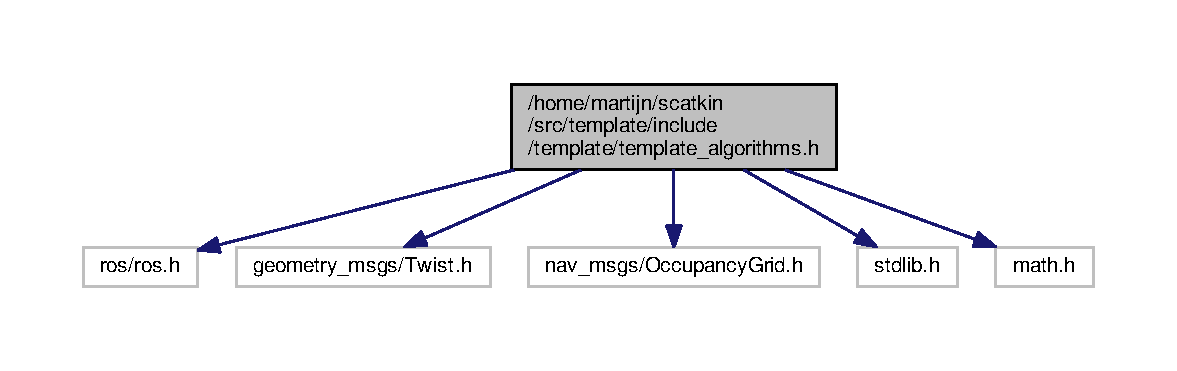
\includegraphics[width=350pt]{template__algorithms_8h__incl}
\end{center}
\end{figure}
This graph shows which files directly or indirectly include this file\+:\nopagebreak
\begin{figure}[H]
\begin{center}
\leavevmode
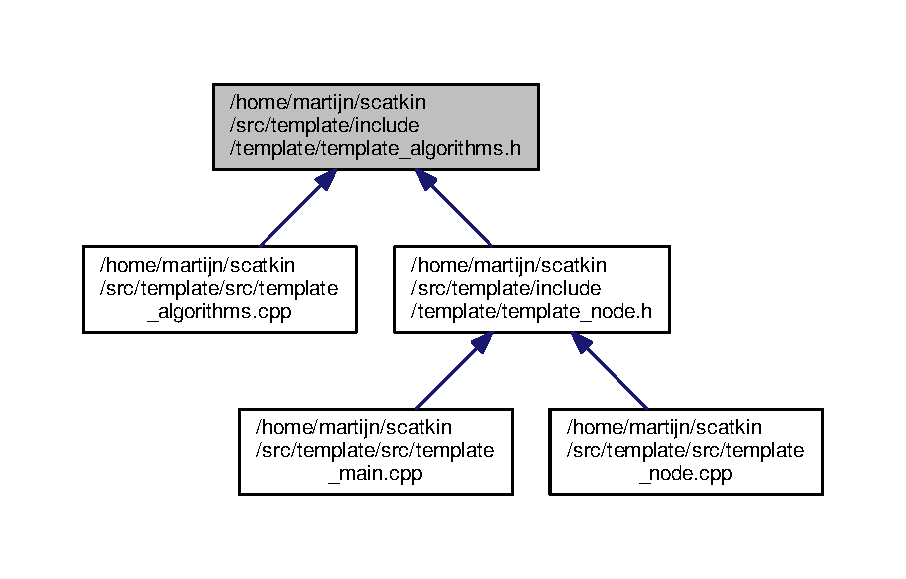
\includegraphics[width=350pt]{template__algorithms_8h__dep__incl}
\end{center}
\end{figure}
\subsection*{Classes}
\begin{DoxyCompactItemize}
\item 
class \hyperlink{classtemplate__node_1_1TemplateAlgorithms}{template\+\_\+node\+::\+Template\+Algorithms}
\end{DoxyCompactItemize}
\subsection*{Namespaces}
\begin{DoxyCompactItemize}
\item 
 \hyperlink{namespacetemplate__node}{template\+\_\+node}
\end{DoxyCompactItemize}

\hypertarget{template__node_8h}{}\section{/home/martijn/scatkin/src/template/include/template/template\+\_\+node.h File Reference}
\label{template__node_8h}\index{/home/martijn/scatkin/src/template/include/template/template\+\_\+node.\+h@{/home/martijn/scatkin/src/template/include/template/template\+\_\+node.\+h}}
{\ttfamily \#include $<$ros/ros.\+h$>$}\\*
{\ttfamily \#include $<$geometry\+\_\+msgs/\+Twist.\+h$>$}\\*
{\ttfamily \#include $<$nav\+\_\+msgs/\+Occupancy\+Grid.\+h$>$}\\*
{\ttfamily \#include $<$stdlib.\+h$>$}\\*
{\ttfamily \#include $<$math.\+h$>$}\\*
{\ttfamily \#include \char`\"{}template/template\+\_\+algorithms.\+h\char`\"{}}\\*
Include dependency graph for template\+\_\+node.\+h\+:\nopagebreak
\begin{figure}[H]
\begin{center}
\leavevmode
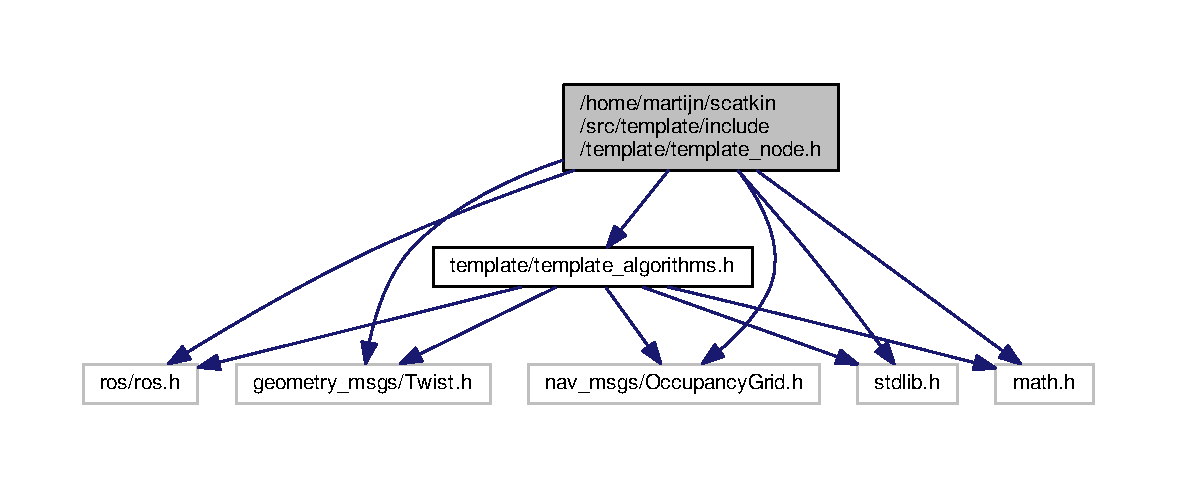
\includegraphics[width=350pt]{template__node_8h__incl}
\end{center}
\end{figure}
This graph shows which files directly or indirectly include this file\+:\nopagebreak
\begin{figure}[H]
\begin{center}
\leavevmode
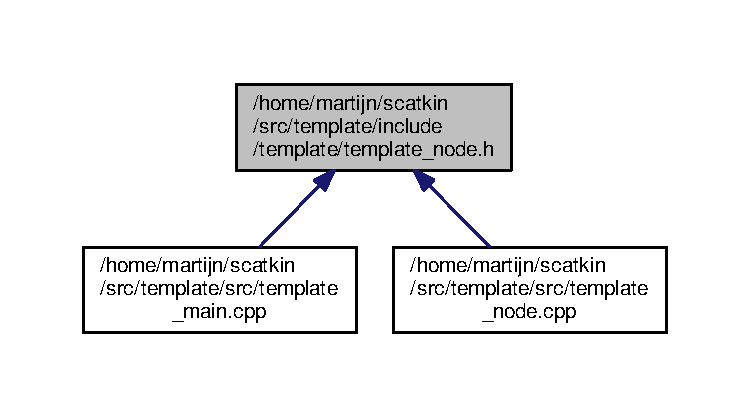
\includegraphics[width=350pt]{template__node_8h__dep__incl}
\end{center}
\end{figure}
\subsection*{Classes}
\begin{DoxyCompactItemize}
\item 
class \hyperlink{classtemplate__node_1_1TemplateNode}{template\+\_\+node\+::\+Template\+Node}
\end{DoxyCompactItemize}
\subsection*{Namespaces}
\begin{DoxyCompactItemize}
\item 
 \hyperlink{namespacetemplate__node}{template\+\_\+node}
\end{DoxyCompactItemize}

\hypertarget{template__algorithms_8cpp}{}\section{/home/martijn/scatkin/src/template/src/template\+\_\+algorithms.cpp File Reference}
\label{template__algorithms_8cpp}\index{/home/martijn/scatkin/src/template/src/template\+\_\+algorithms.\+cpp@{/home/martijn/scatkin/src/template/src/template\+\_\+algorithms.\+cpp}}
{\ttfamily \#include \char`\"{}template/template\+\_\+algorithms.\+h\char`\"{}}\\*
Include dependency graph for template\+\_\+algorithms.\+cpp\+:\nopagebreak
\begin{figure}[H]
\begin{center}
\leavevmode
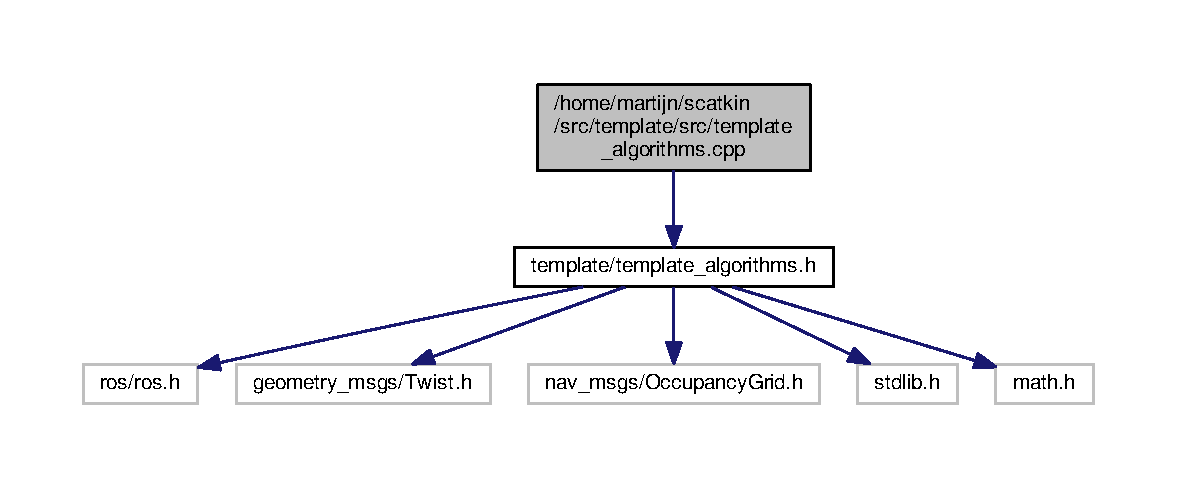
\includegraphics[width=350pt]{template__algorithms_8cpp__incl}
\end{center}
\end{figure}
\subsection*{Namespaces}
\begin{DoxyCompactItemize}
\item 
 \hyperlink{namespacetemplate__node}{template\+\_\+node}
\end{DoxyCompactItemize}

\hypertarget{template__main_8cpp}{}\section{/home/martijn/scatkin/src/template/src/template\+\_\+main.cpp File Reference}
\label{template__main_8cpp}\index{/home/martijn/scatkin/src/template/src/template\+\_\+main.\+cpp@{/home/martijn/scatkin/src/template/src/template\+\_\+main.\+cpp}}
{\ttfamily \#include \char`\"{}template/template\+\_\+node.\+h\char`\"{}}\\*
Include dependency graph for template\+\_\+main.\+cpp\+:\nopagebreak
\begin{figure}[H]
\begin{center}
\leavevmode
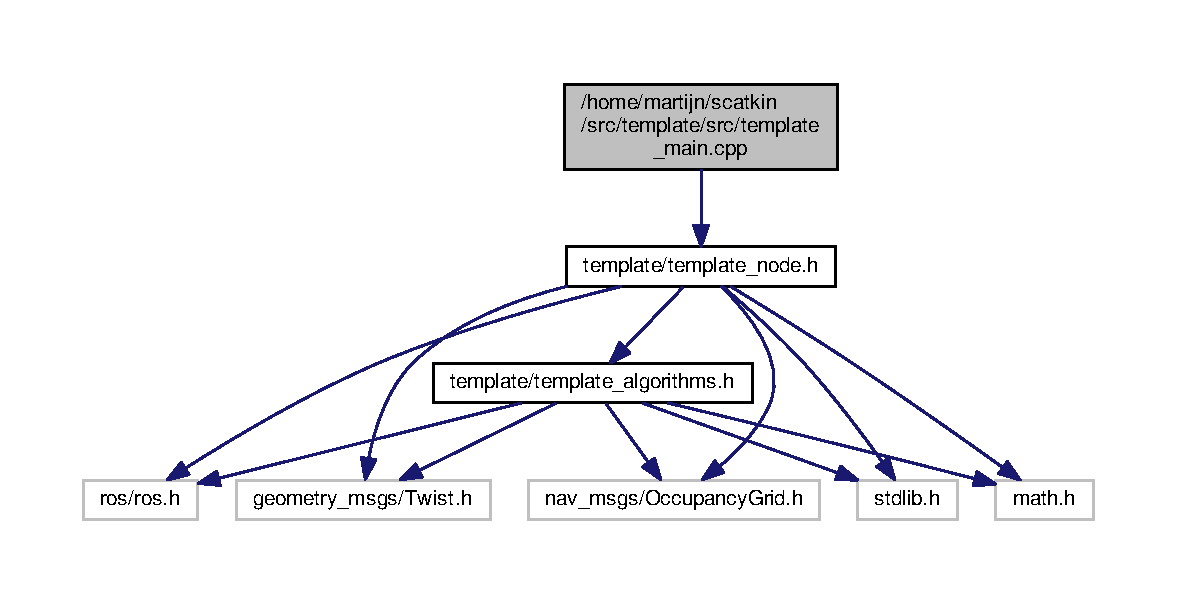
\includegraphics[width=350pt]{template__main_8cpp__incl}
\end{center}
\end{figure}
\subsection*{Functions}
\begin{DoxyCompactItemize}
\item 
int \hyperlink{template__main_8cpp_a3c04138a5bfe5d72780bb7e82a18e627}{main} (int argc, char $\ast$$\ast$argv)
\end{DoxyCompactItemize}


\subsection{Function Documentation}
\index{template\+\_\+main.\+cpp@{template\+\_\+main.\+cpp}!main@{main}}
\index{main@{main}!template\+\_\+main.\+cpp@{template\+\_\+main.\+cpp}}
\subsubsection[{\texorpdfstring{main(int argc, char $\ast$$\ast$argv)}{main(int argc, char **argv)}}]{\setlength{\rightskip}{0pt plus 5cm}int main (
\begin{DoxyParamCaption}
\item[{int}]{argc, }
\item[{char $\ast$$\ast$}]{argv}
\end{DoxyParamCaption}
)}\hypertarget{template__main_8cpp_a3c04138a5bfe5d72780bb7e82a18e627}{}\label{template__main_8cpp_a3c04138a5bfe5d72780bb7e82a18e627}
When debugging, set logger\+\_\+level to Debug by changing Info to Debug. 
\hypertarget{template__node_8cpp}{}\section{/home/martijn/scatkin/src/template/src/template\+\_\+node.cpp File Reference}
\label{template__node_8cpp}\index{/home/martijn/scatkin/src/template/src/template\+\_\+node.\+cpp@{/home/martijn/scatkin/src/template/src/template\+\_\+node.\+cpp}}
{\ttfamily \#include \char`\"{}template/template\+\_\+node.\+h\char`\"{}}\\*
Include dependency graph for template\+\_\+node.\+cpp\+:\nopagebreak
\begin{figure}[H]
\begin{center}
\leavevmode
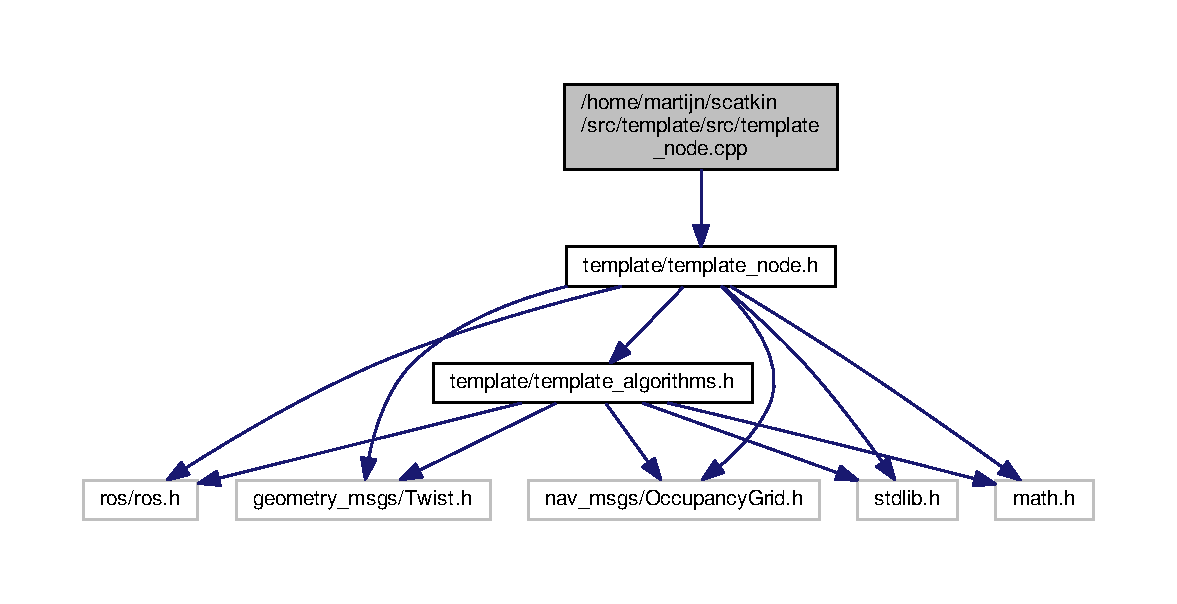
\includegraphics[width=350pt]{template__node_8cpp__incl}
\end{center}
\end{figure}
\subsection*{Namespaces}
\begin{DoxyCompactItemize}
\item 
 \hyperlink{namespacetemplate__node}{template\+\_\+node}
\end{DoxyCompactItemize}

%--- End generated contents ---

% Index
\backmatter
\newpage
\phantomsection
\clearemptydoublepage
\addcontentsline{toc}{chapter}{Index}
\printindex

\end{document}
